\section{\logtitle 11/24-2015} % Remember to set
\duration{9:00}{16:00}
\attend{\at}{\at}{\at}{\at}


\begin{itemize}
	\item [\textbf{Meeting pins:}]
	\item Implement code skeleton feedback
	\item Connect implementation tasks with functional requirements
	\item Fix UWP vs standard application issue 
\end{itemize}

\begin{itemize}
	\item [\textbf{Sprint Planning:}]
	\item Need to fix subsystem dependencies with TAs by possibly using 
	\item Connect functional requirements with implementation tasks
	\item Plan coding tasks for the next 4 weeks 
\end{itemize}

\newpage

\textbf{Implementation priorities based on functional requirements subsystem dependencies:}

\textbf{Application logic}
\begin{itemize}
	\item UserManagement will be implemented first because WebApi and StudyManagement depend on it. We need to define how a User is to be represented so that SM can use WA. 
	\item StudyManagement should be implemented secondly because its criteria and phase classes are used to define a study configuration. ProtocolManagement depends on a finalized study configuration.
	\item ExportManagement and PaperManagement can be implemented independently from rest of project. 
	\item All subsystems depends on Repository with predefined CRUD operations.
	\item WebAPI depends on all subsystems based on their methods. We need to define what methods each package handler holds in order to develop our WebApi. The WebApi will be based on the deliveries from Steven. 
\end{itemize} 

\textbf{Interface}
\begin{itemize}
	\item StudyConfigurationUI is independent from all subsystems in application logic. It is based on a web api that uses the server in the application logic. Should be able to retrieve teams stored in database and create a study define passed to the application logic. 
\end{itemize} 

\textbf{User Validation}
The application logic will not handle user validation (e.g. manager or researcher), which is handled in the interface part of the system between yellow and blue part. The only thing application logic considers is whether a given user exists in the database. Roles are checked in Study Management based on an enum flagtype related to a user, e.g. a user can have a "Reviewer", "Manager" or "Validator" role determining which tasks are to be returned. A Reviewer will receive review tasks and a Validator will receive conflict tasks. Blue team will validate users based on whether they represent a Manager or Researcher. 

\newpage

\textbf{Code Skeleton Design Changed to reduce coupling}

If all packages have a facade interface used by other subsystems it allows single responsibility. Also allows team members to work on subsystems independently. We do not touch each other's code this way. A sub system should be able to be pulled out and replaced without causing trouble. By way of example, ExportManagement depends on the ProtocolManagement and its a predefined protocol. A using statement for Protocol is used in ExportManagement. Thus, we need to change the UML and use a dashed line between ExportManagement and ProtocolManagement. The dependency resides in where the object comes from and not how it is passed (e.g. from WebAPI). 

\begin{figure}[H]
	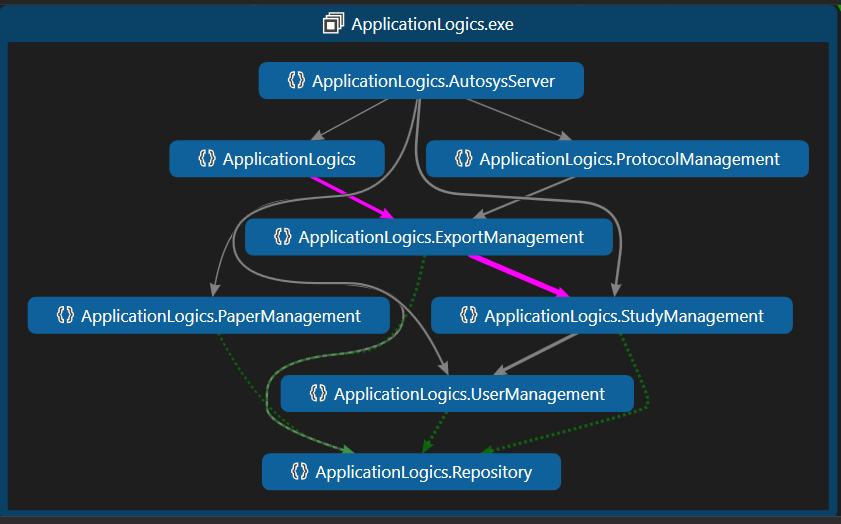
\includegraphics[width = 31 em]{image/oldsubsystemdependencies}
	\label{fig:Subsystem Dependencies}
	\caption{Subsystem Dependencies}
\end{figure}
